\subsection{Alcance del marco y articulación con los objetivos}
El desarrollo de un instrumento virtual geoespacial orientado al análisis de la accidentalidad vial implica abordar el problema desde una perspectiva interdisciplinaria en la que convergen la ingeniería de software, los sistemas de información geográfica, la ciencia de datos y la analítica de indicadores. Esta integración permite transformar registros dispersos en información estructurada y generar conocimiento útil para la toma de decisiones en seguridad vial. En \textbf{ViaData — Medellín}, el sistema no se limita a almacenar datos: actúa como plataforma analítica capaz de representar, procesar y visualizar patrones espaciales y temporales, en línea con enfoques recientes que vinculan analítica territorial y gobernanza del dato en seguridad vial \cite{oms2024,monar2025}.

El objetivo general plantea un instrumento que permita \textbf{visualizar, analizar y segmentar} información de accidentalidad, apoyado en modelos estadísticos para decisiones en seguridad vial. Los objetivos específicos exigen: \textbf{(i)} arquitectura y modelo de datos geoespacial; \textbf{(ii)} módulos de análisis estadístico para índices por comuna, franja horaria, tipo de vehículo y gravedad; \textbf{(iii)} tablero de monitoreo y diagnóstico; y \textbf{(iv)} validación técnica del desempeño y la calidad del software. En consecuencia, el marco conceptual articula \textbf{ingeniería de software aplicada} (monolito Django con API REST y cliente React), \textbf{SIG y bases de datos espaciales}, \textbf{ciencia de datos con analítica descriptiva, diagnóstica y predictiva} ---implementada con modelos estadísticos transparentes y validación \textit{hold-out}---, y \textbf{medición territorial} mediante indicadores codificados (familias G y P) y agregaciones espacio-temporales. Esta lectura es coherente con los antecedentes del documento sobre mapas de calor, focalización territorial y calidad de la información \cite{parraga2024,oviedo2025}.

\subsection{Desarrollo de software: arquitectura monolítica con Django}
En ingeniería de software, la \textbf{arquitectura} condiciona mantenibilidad, despliegue y seguridad. Frente a un despliegue totalmente distribuido en microservicios, el \textbf{patrón monolítico} adoptado en ViaData — Medellín concentra en un único backend la autenticación JWT, la \textbf{API REST} (Django REST Framework), la lógica de negocio analítica y el acceso a datos, mientras el frontend React (Vite) opera como aplicación de página única que consume esos servicios. Esta organización reduce la complejidad de despliegue en un contexto de grado y mantiene trazable el vínculo entre indicadores expuestos en la interfaz y el código que los calcula \cite{lugo2025}.

El framework Django estructura el proyecto en capas compatibles con el patrón \textbf{modelo–vista–plantilla} (MVT), favoreciendo separación de responsabilidades. \textbf{Django REST Framework} expone los endpoints que alimentan tablero, mapa, predicciones, reportes y asistente conversacional. \textbf{GeoDjango} y PostgreSQL con extensión \textbf{PostGIS} habilitan geometrías, asignación territorial y consultas espaciales. La calidad se refuerza con pruebas automatizadas (\texttt{pytest}, \texttt{pytest-django}), coherente con el objetivo específico de validar desempeño y seguridad del software.

\begin{figure}[H]
	\centering
	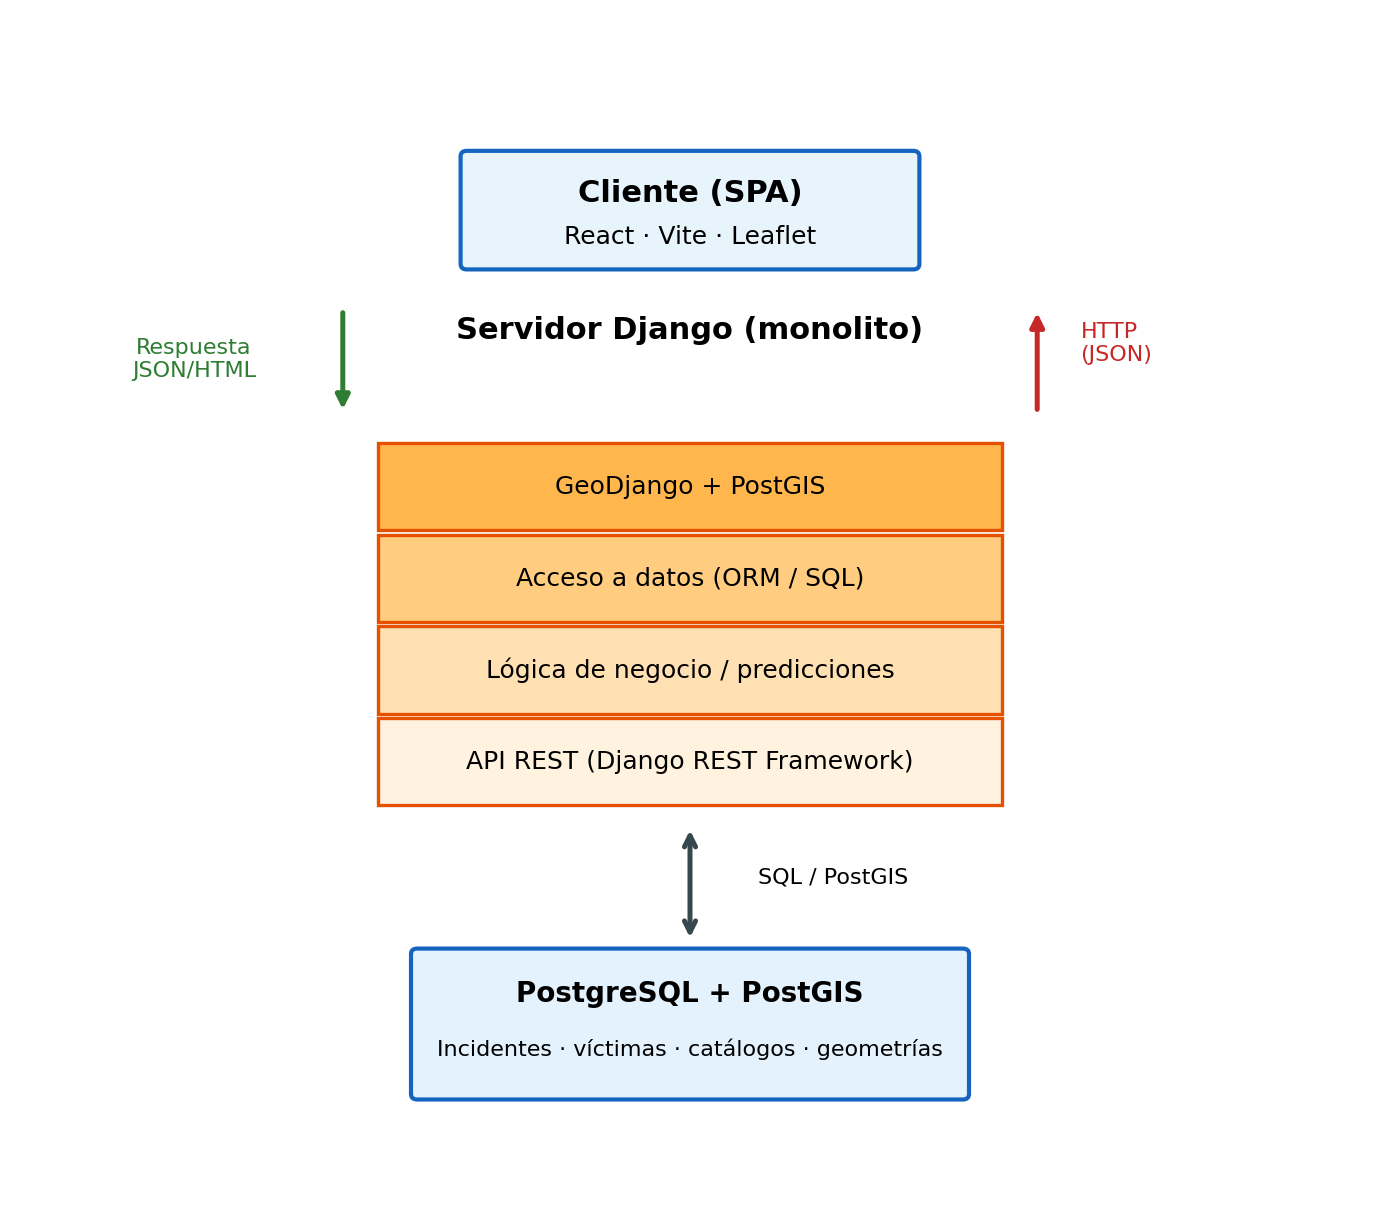
\includegraphics[width=0.75\linewidth]{images/fig_arquitectura_mtv.png}
	\caption{Patrón repositorio MTV en el backend de ViaData — Medellín}
	\label{fig:arquitectura-monolitica}
\end{figure}

\subsection{Sistemas de información geográficos y análisis espacial urbano}
Los \textbf{SIG} integran datos georreferenciados con atributos descriptivos (tipo de incidente, gravedad, franja horaria, entre otros), lo que permite estudiar \textbf{patrones territoriales y zonas críticas}. La literatura aplicada sostiene que los siniestros tienden a concentrarse en corredores e intersecciones asociados a infraestructura, flujo y comportamiento. Técnicas como la \textbf{estimación de densidad por núcleo} (KDE) y el \textbf{análisis de agrupación espacial} se emplean para identificar puntos calientes y priorizar intervenciones \cite{xu2022,li2023}.

\textbf{PostGIS} aporta tipos y operadores espaciales (\texttt{ST\_Contains}, índices espaciales); \textbf{GeoDjango} acerca esa capacidad al dominio de la aplicación. En el cliente, \textbf{Leaflet} y \textbf{react-leaflet} materializan capas de puntos, densidad y coroplética a partir de agregaciones del backend. ViaData — Medellín distingue además un \textbf{modo de territorio registro} ---filtro por comuna o barrio declarado en el registro Mede--- y un \textbf{modo espacial} ---asignación por polígono oficial a partir de coordenadas---, lo que permite contrastar la calidad cartográfica del dato mediante el indicador G03.

\begin{figure}[H]
	\centering
	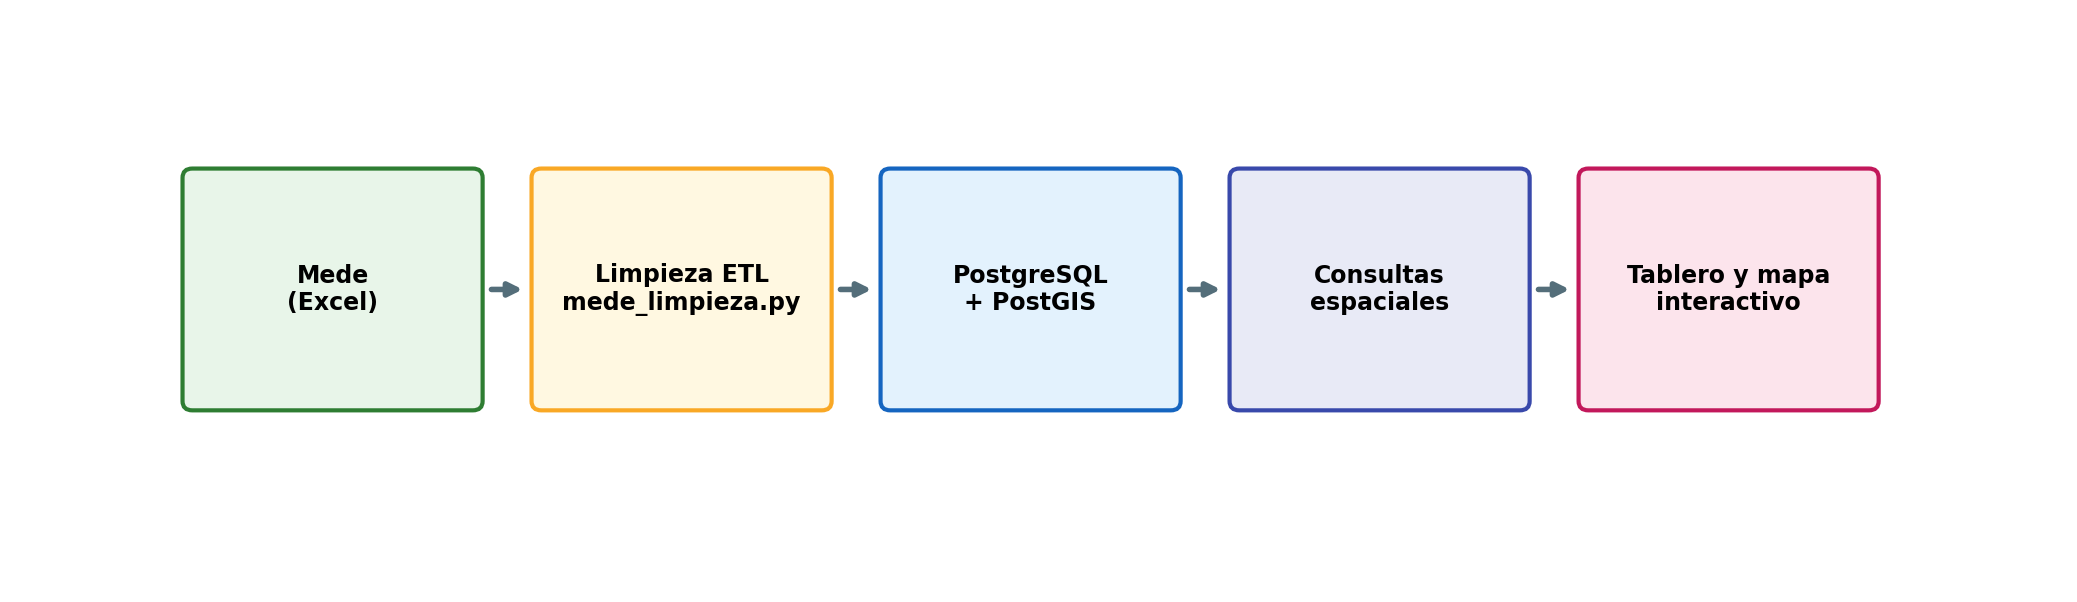
\includegraphics[width=0.95\linewidth]{images/fig_flujo_datos_geoespacial.png}
	\caption{Ciclo de vida de los datos geoespaciales (origen--destino)}
	\label{fig:flujo-de-datos-geoespacial}
\end{figure}

\subsection{Definiciones operativas en ViaData — Medellín}
Para evitar ambigüedades entre el lenguaje cotidiano de la seguridad vial y los cálculos del sistema, se adoptan las siguientes definiciones operativas:

\begin{table}[H]
	\centering
	\caption{Definiciones operativas del sistema}
	\label{tab:definiciones-operativas}
	\small
	\begin{tabularx}{\linewidth}{@{}l X@{}}
		\toprule
		\textbf{Término} & \textbf{Definición en ViaData — Medellín} \\
		\midrule
		Incidente & Evento de siniestro vial registrado en Mede; unidad de conteo distinta por identificador de incidente. \\
		Víctima & Persona asociada a un incidente; puede haber varias por evento. \\
		Víctima fatal & Clasificación según catálogo de gravedad (fatal, muerte, entre otras categorías equivalentes). \\
		Proyección & Escenario orientativo bajo estabilidad del patrón histórico filtrado; no implica causalidad. \\
		Hold-out & Validación que reserva los últimos meses del rango, entrena sin ellos y mide error al predecirlos. \\
		Participación por día & Porcentaje de incidentes en un día respecto al total del periodo; no es probabilidad individual. \\
		Modo registro / espacial & Filtro territorial por atributo declarado en Mede o por polígono PostGIS, respectivamente. \\
		\bottomrule
	\end{tabularx}
\end{table}

\clearpage

\subsection{Ciencia de datos, indicadores y tipos de modelos}
La ciencia de datos articula estadística, computación y dominio para convertir registros operativos en evidencia útil. En este proyecto el flujo incluye ingestión desde el Excel Mede, depuración centralizada, asociación a catálogos normalizados y carga a PostgreSQL/PostGIS; el análisis en tiempo de consulta combina SQL parametrizado y rutinas en NumPy. La solidez del análisis depende de la calidad del dato y de su integración con contexto territorial y temporal \cite{provost2022,atancuri2024}.

\subsubsection{Indicadores y analítica descriptiva / diagnóstica}
La medición de la siniestralidad se expresa en indicadores temporales, espaciales y de gravedad (frecuencia, severidad, tendencia). En el tablero y el mapa de ViaData — Medellín, KPIs, series mensuales, matrices día$\times$hora y rankings por comuna o barrio permiten la lectura diagnóstica del periodo seleccionado. El \textbf{índice de prioridad territorial P05} ---ponderación de frecuencia (30\,\%), densidad (15\,\%), tendencia (20\,\%), componente fatal (20\,\%) y participación relativa (15\,\%)--- materializa la lógica de priorización multicriterio sin recurrir a catálogos de vía o punto crítico, ausentes en la fuente Mede cargada \cite{parraga2024}.

\begin{figure}[H]
	\centering
	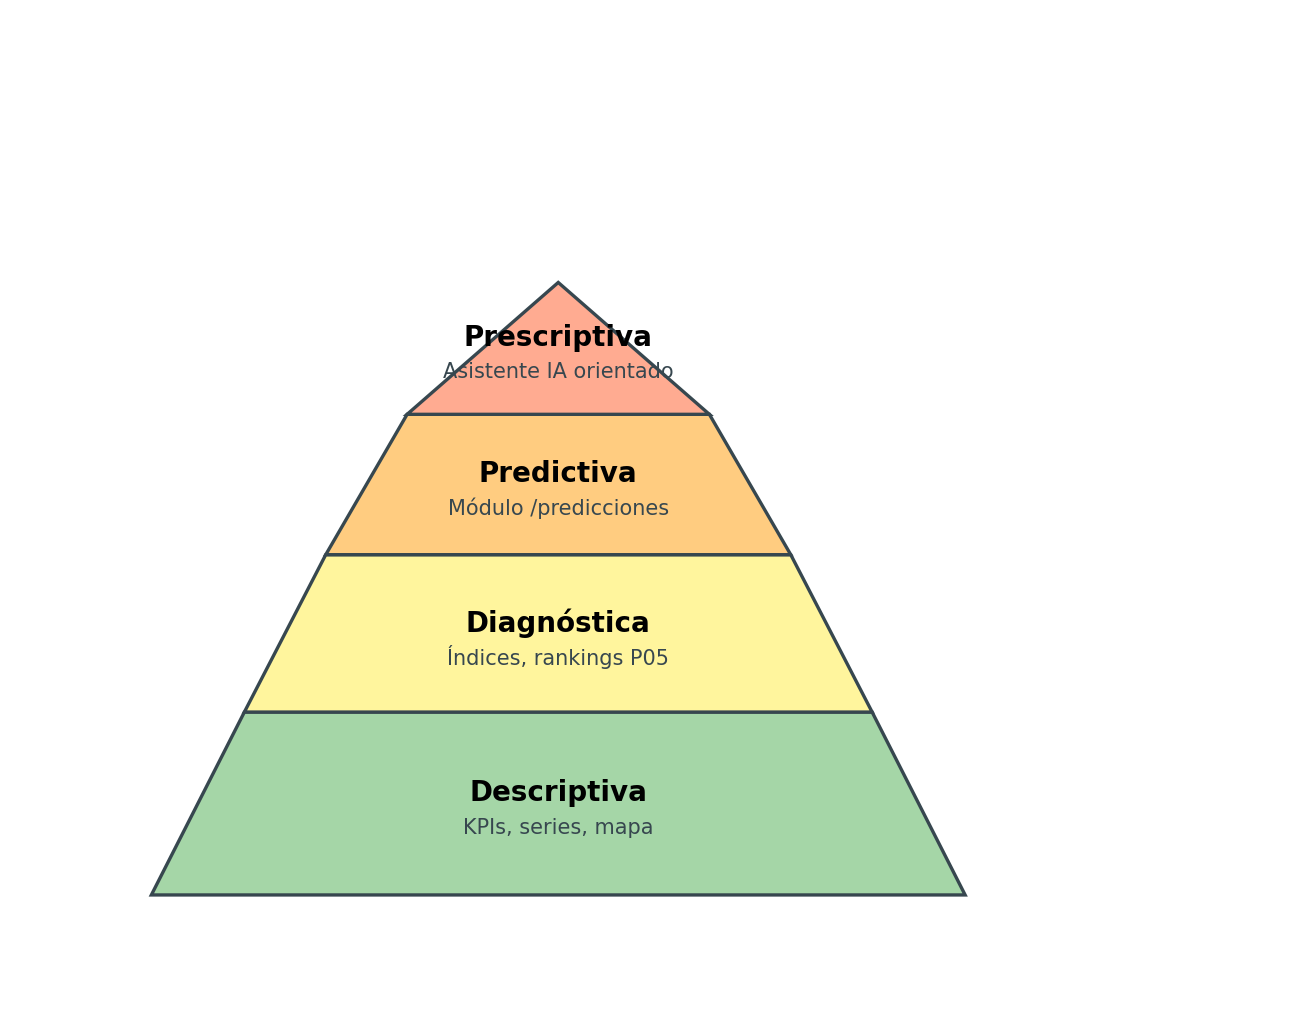
\includegraphics[width=0.8\linewidth]{images/fig_taxonomia_analitica.png}
	\caption{Taxonomía de analítica en ViaData — Medellín}
	\label{fig:arquitectura-monolitica-pagina-3}
\end{figure}

\subsubsection{Modelado de conteos y series temporales}
Los accidentes agregados por mes son variables de \textbf{conteo} con posible sobredispersión y estacionalidad intra-anual. En la literatura de accidentalidad se emplean, entre otros, modelos de \textbf{regresión de Poisson} o binomial negativa, \textbf{regresión lineal (OLS)} como línea base interpretable, y \textbf{ARIMA/SARIMA} cuando importa la memoria temporal y la estacionalidad mensual. ViaData — Medellín implementa variantes comparables en la interfaz ---OLS, diseño estacional, Poisson log-lineal, media móvil, bandas $\mu \pm 3\sigma$, ARIMA y SARIMA--- priorizando interpretabilidad y validación predictiva sobre modelos de caja negra \cite{lugo2025}.

Las series mensuales de Medellín combinan tendencia, estacionalidad y \textbf{shocks} estructurales ---como el confinamiento de mar–ago 2020---, por lo que el ajuste predictivo admite excluir esos meses del entrenamiento. Para proporciones ---porcentaje de víctimas fatales--- se requieren formulaciones distintas: regresión estacional sobre el porcentaje, \textbf{logit con exposición} o \textbf{ratio compuesto} al proyectar fatales y víctimas por separado.

\subsubsection{Validación predictiva: in-sample y hold-out}
El ajuste \textbf{in-sample} mide qué tan bien el modelo reproduce el periodo con el que fue estimado (R², MAPE in-sample), pero puede sobrevalorar modelos complejos. El esquema \textbf{hold-out} reserva los últimos $N$ meses del rango, entrena sin ellos y calcula el error al predecirlos; en ViaData — Medellín es el \textbf{criterio principal} para elegir modelo en proyección mensual y proporción de fatales. Se adopta como umbral exploratorio un MAPE hold-out $\leq 20\,\%$ (precisión estimada $\approx 100\,\% - \mathrm{MAPE}$), sin exigir R² $\geq 0{,}80$ en series mensuales perturbadas por la pandemia.

\begin{figure}[H]
	\centering
	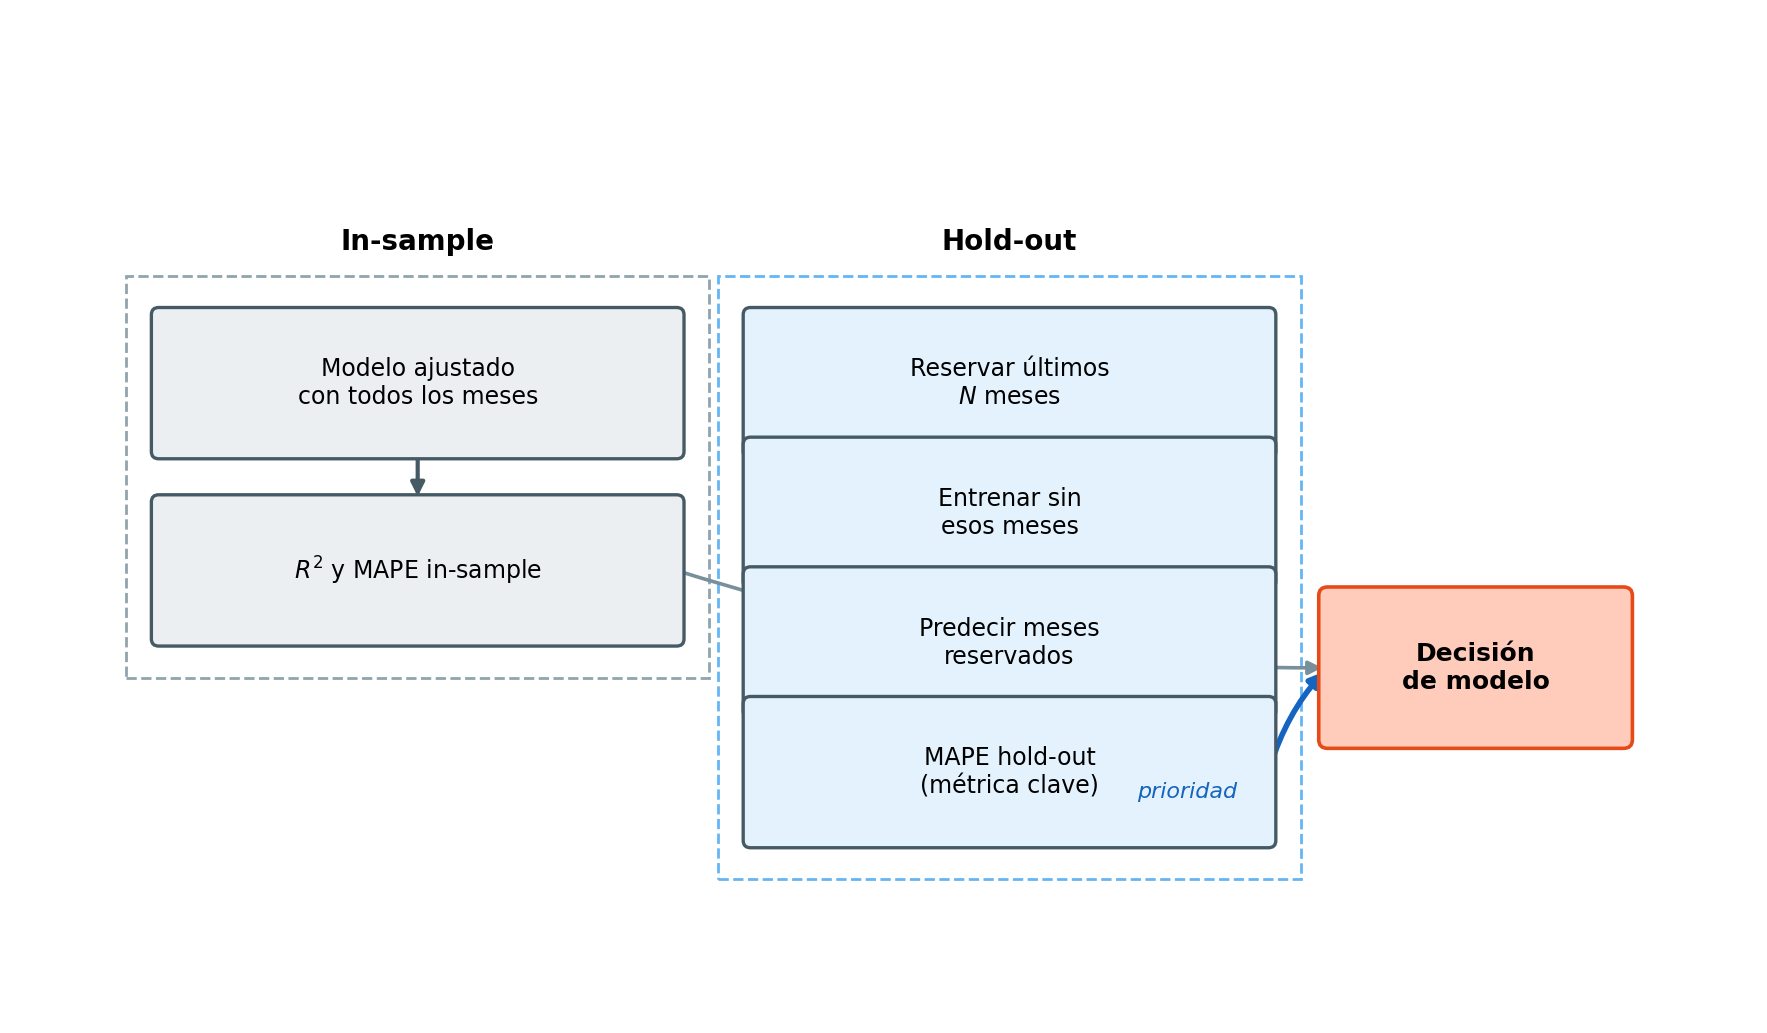
\includegraphics[width=0.90\linewidth]{images/fig_holdout_validacion.png}
	\caption{Esquema de validación in-sample frente a hold-out en el módulo de predicciones}
	\label{fig:holdout-validacion}
\end{figure}

\subsubsection{Familias de modelos en la plataforma}
\begin{itemize}[]
	\item \textbf{Formulaciones explícitas} (tasas, promedios, ponderaciones en SQL o servicios Django) actúan como modelos cerrados a escala de indicador, útiles en tablero y mapa.
	\item \textbf{Modelos empíricos y estadísticos} se apoyan en la historia operativa: agregaciones multidimensionales, comparación de periodos e índice P05, calculado como $0{,}30\,s_{\text{freq}} + 0{,}15\,s_{\text{dens}} + 0{,}20\,s_{\text{tend}} + 0{,}20\,s_{\text{fatal}} + 0{,}15\,s_{\text{part}}$ (cada $s$ en escala 0--100 dentro del territorio filtrado).
	\item \textbf{Modelos predictivos de series} se implementan con NumPy en rutinas propias (OLS, estacional, Poisson, media móvil, $\mu \pm 3\sigma$) y con \textbf{statsmodels} para ARIMA/SARIMA; no se emplean \texttt{scikit-learn} ni redes neuronales, por decisión de alcance orientada a transparencia y reproducibilidad.
\end{itemize}
Técnicas espaciales como KDE o cuadrículas de concentración (hotspots P14) complementan la lectura territorial cuando el volumen y la resolución del dato lo permiten \cite{xu2022,monar2025}.

\subsection{Taxonomía de indicadores del sistema}
Los indicadores de ViaData — Medellín se organizan en dos familias: \textbf{G} (geoespaciales y de calidad) y \textbf{P} (predictivos y de priorización). La Tabla~\ref{tab:taxonomia-indicadores} resume su propósito; el detalle de fórmulas y evaluación se presenta en metodología y resultados.

\begin{table}[H]
	\centering
	\caption{Taxonomía de indicadores G y P}
	\label{tab:taxonomia-indicadores}
	\small
	\begin{tabularx}{\linewidth}{@{}l l X@{}}
		\toprule
		\textbf{ID} & \textbf{Módulo} & \textbf{Pregunta analítica} \\
		\midrule
		G01--G02 & Mapa / tablero & Densidad de incidentes por km² \\
		G03 & Mapa / tablero & Coincidencia entre territorio registro y espacial \\
		G06 / P14 & Mapa & Concentración espacial (top celdas / hotspots) \\
		P01--P04 & Predicciones §1 & ¿Cuántos incidentes, víctimas o fatales por mes? \\
		P05 & Predicciones §2 & ¿Qué territorio priorizar en el periodo filtrado? \\
		P08--P10 & Predicciones §3 & ¿Qué territorio concentrará carga futura? \\
		P07 & Predicciones §4 & ¿Cómo evoluciona el \% de víctimas fatales? \\
		P12--P13 & Predicciones §5 & ¿Cuándo se concentrarían los incidentes (día y hora)? \\
		\bottomrule
	\end{tabularx}
\end{table}

\clearpage

\subsection{Roles, permisos y articulación del módulo predictivo}
El acceso a funcionalidades sigue un esquema de roles almacenado en perfil de usuario. Ciudadanos y visitantes sin autenticación consultan tablero, mapa y asistente con herramientas descriptivas; analistas y administradores acceden además a predicciones y reportes; solo el administrador gestiona cuentas. El rol autoridad se reserva para extensiones institucionales.

Los cinco bloques del módulo predictivo comparten filtros de fechas, territorio, clase de incidente y exclusión opcional de meses COVID, pero responden preguntas distintas. La proyección mensual (§1) alimenta el total de horizonte para patrones día$\times$hora (§5); la prioridad territorial (§2) mira el pasado reciente; la carga esperada (§3) orienta el ranking futuro por comuna o barrio; la proporción de fatales (§4) aporta el componente de gravedad relativa al índice P05. El diagrama de la Figura~\ref{fig:cadena-predictiva} resume esas dependencias conceptuales.

\begin{figure}[H]
	\centering
	\resizebox{\linewidth}{!}{%
	\begin{tikzpicture}[
		node distance=0.45cm and 0.5cm,
		mod/.style={draw, rounded corners, align=center, font=\scriptsize, inner sep=3pt, minimum width=2.4cm},
		filt/.style={draw, dashed, rounded corners, align=center, font=\scriptsize, inner sep=4pt, minimum width=5.8cm},
		arr/.style={-{Stealth[length=1.8mm]}, thick},
		darr/.style={-{Stealth[length=1.8mm]}, thick, dashed}
	]
		\node[filt] (f) {Filtros: fechas, territorio, clase, COVID};
		\node[mod, fill=blue!10, below left=1cm and 0.1cm of f] (s1) {§1 Proyección\\mensual};
		\node[mod, fill=green!12, below=1cm of f] (s2) {§2 Prioridad\\P05};
		\node[mod, fill=green!12, below right=1cm and 0.1cm of f] (s3) {§3 Carga\\territorial};
		\node[mod, fill=yellow!15, below left=1cm and 0.1cm of s1] (s4) {§4 \%\\fatales};
		\node[mod, fill=orange!12, below right=1cm and 0.1cm of s3] (s5) {§5 Patrones\\día$\times$hora};
		\draw[arr] (f) -- (s1); \draw[arr] (f) -- (s2);
		\draw[arr] (f) -- (s3); \draw[arr] (f) -- (s4); \draw[arr] (f) -- (s5);
		\draw[arr] (s1) -- node[above, font=\tiny, sloped] {total} (s5);
		\draw[darr] (s4) -- node[left, font=\tiny] {fatal} (s2);
		\draw[darr] (s2) -- node[below, font=\tiny] {ranking} (s3);
	\end{tikzpicture}%
	}
	\caption{Cadena conceptual de los bloques predictivos en ViaData — Medellín}
	\label{fig:cadena-predictiva}
\end{figure}

\subsubsection{Consulta en lenguaje natural}
El asistente conversacional incorpora un modelo de lenguaje (Google Gemini) con \textbf{function calling}: el sistema de diálogo selecciona herramientas que invocan las mismas rutas analíticas del backend, en lugar de generar SQL libre o cifras sin trazabilidad. Este enfoque separa la interacción en lenguaje natural del motor de cálculo y reduce el riesgo de respuestas numéricas inconsistentes \cite{carrillo2024}.

\clearpage

\subsection{Modelado de datos para analítica: estrella y copo de nieve}
En inteligencia de negocios y almacenes analíticos, \textbf{el modelo estrella} centraliza métricas en una tabla de hechos (p. ej., incidentes) y la rodea de dimensiones (tiempo, ubicación, tipo de evento). \textbf{El modelo copo de nieve} normaliza dimensiones en subdimensiones, reduciendo redundancia a cambio de consultas más complejas. La selección depende del equilibrio entre rendimiento, escalabilidad y mantenibilidad \cite{londono2024}.

En este trabajo el \textbf{esquema operacional} en PostgreSQL sigue un \textbf{modelo relacional normalizado} (catálogos, \texttt{incidente}, \texttt{victima}, vínculos geográficos), cercano al espíritu de un copo de nieve en las dimensiones de catálogo, mientras que las consultas tipo \textbf{OLAP} (conteos por fechas, comunas, clases) simulan hechos y dimensiones sin imponer un almacén separado. Si en el futuro se materializaran vistas analíticas dedicadas, el modelo estrella sería la referencia para exponer KPIs.

\begin{figure}[H]
	\centering
	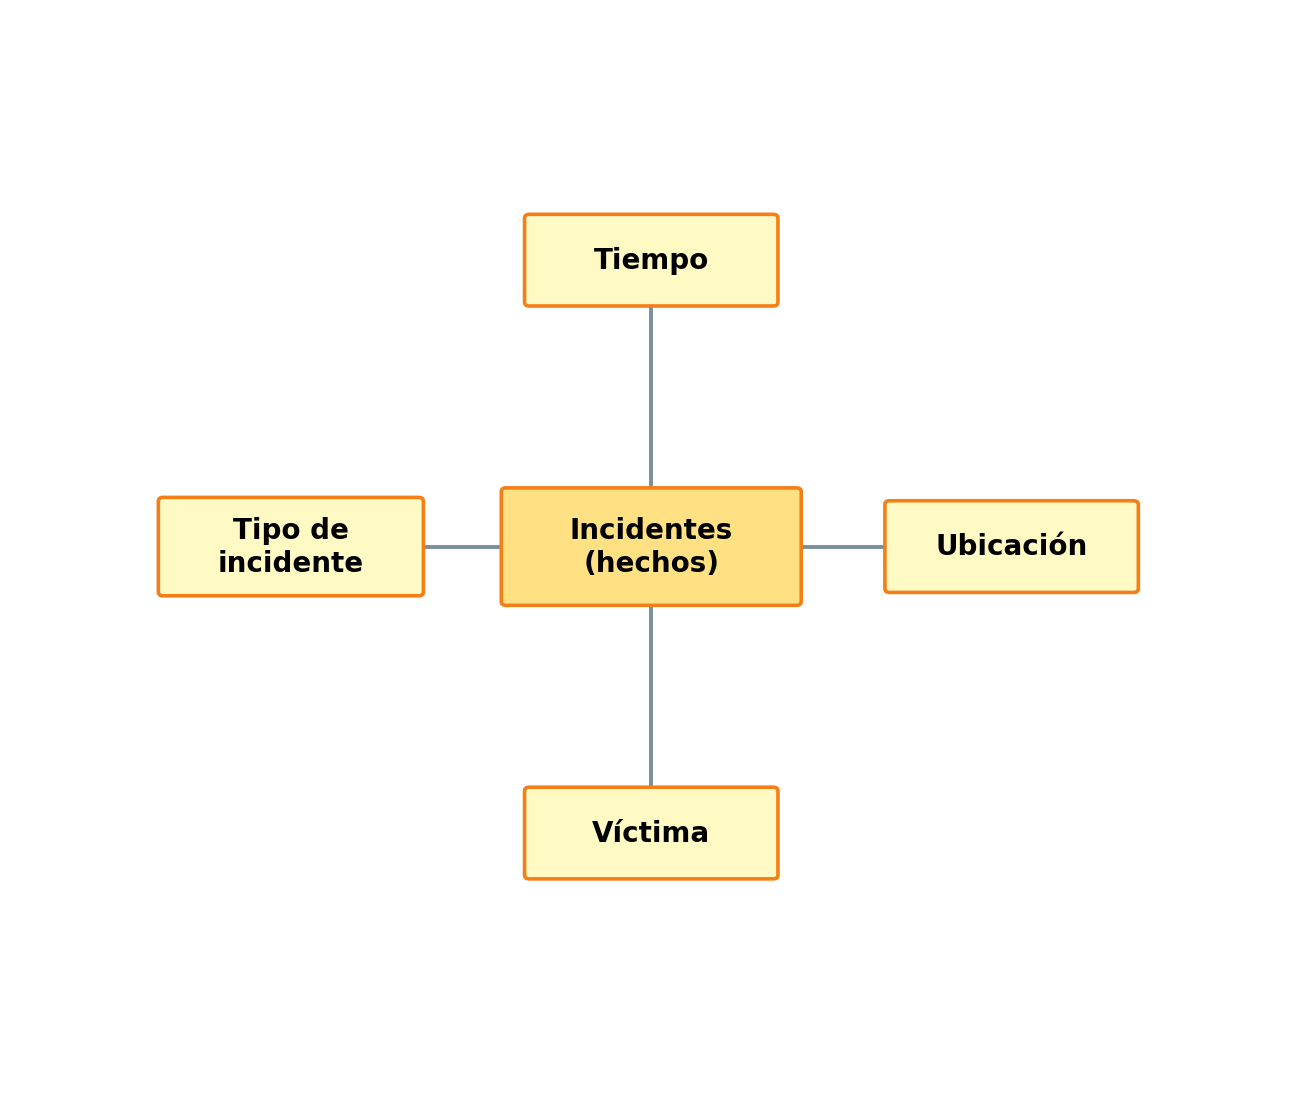
\includegraphics[width=0.65\linewidth]{images/fig_modelo_estrella.png}
	\caption{Modelo estrella (referencia conceptual)}
	\label{fig:arquitectura-monolitica-pagina-4}
\end{figure}

\begin{figure}[H]
	\centering
	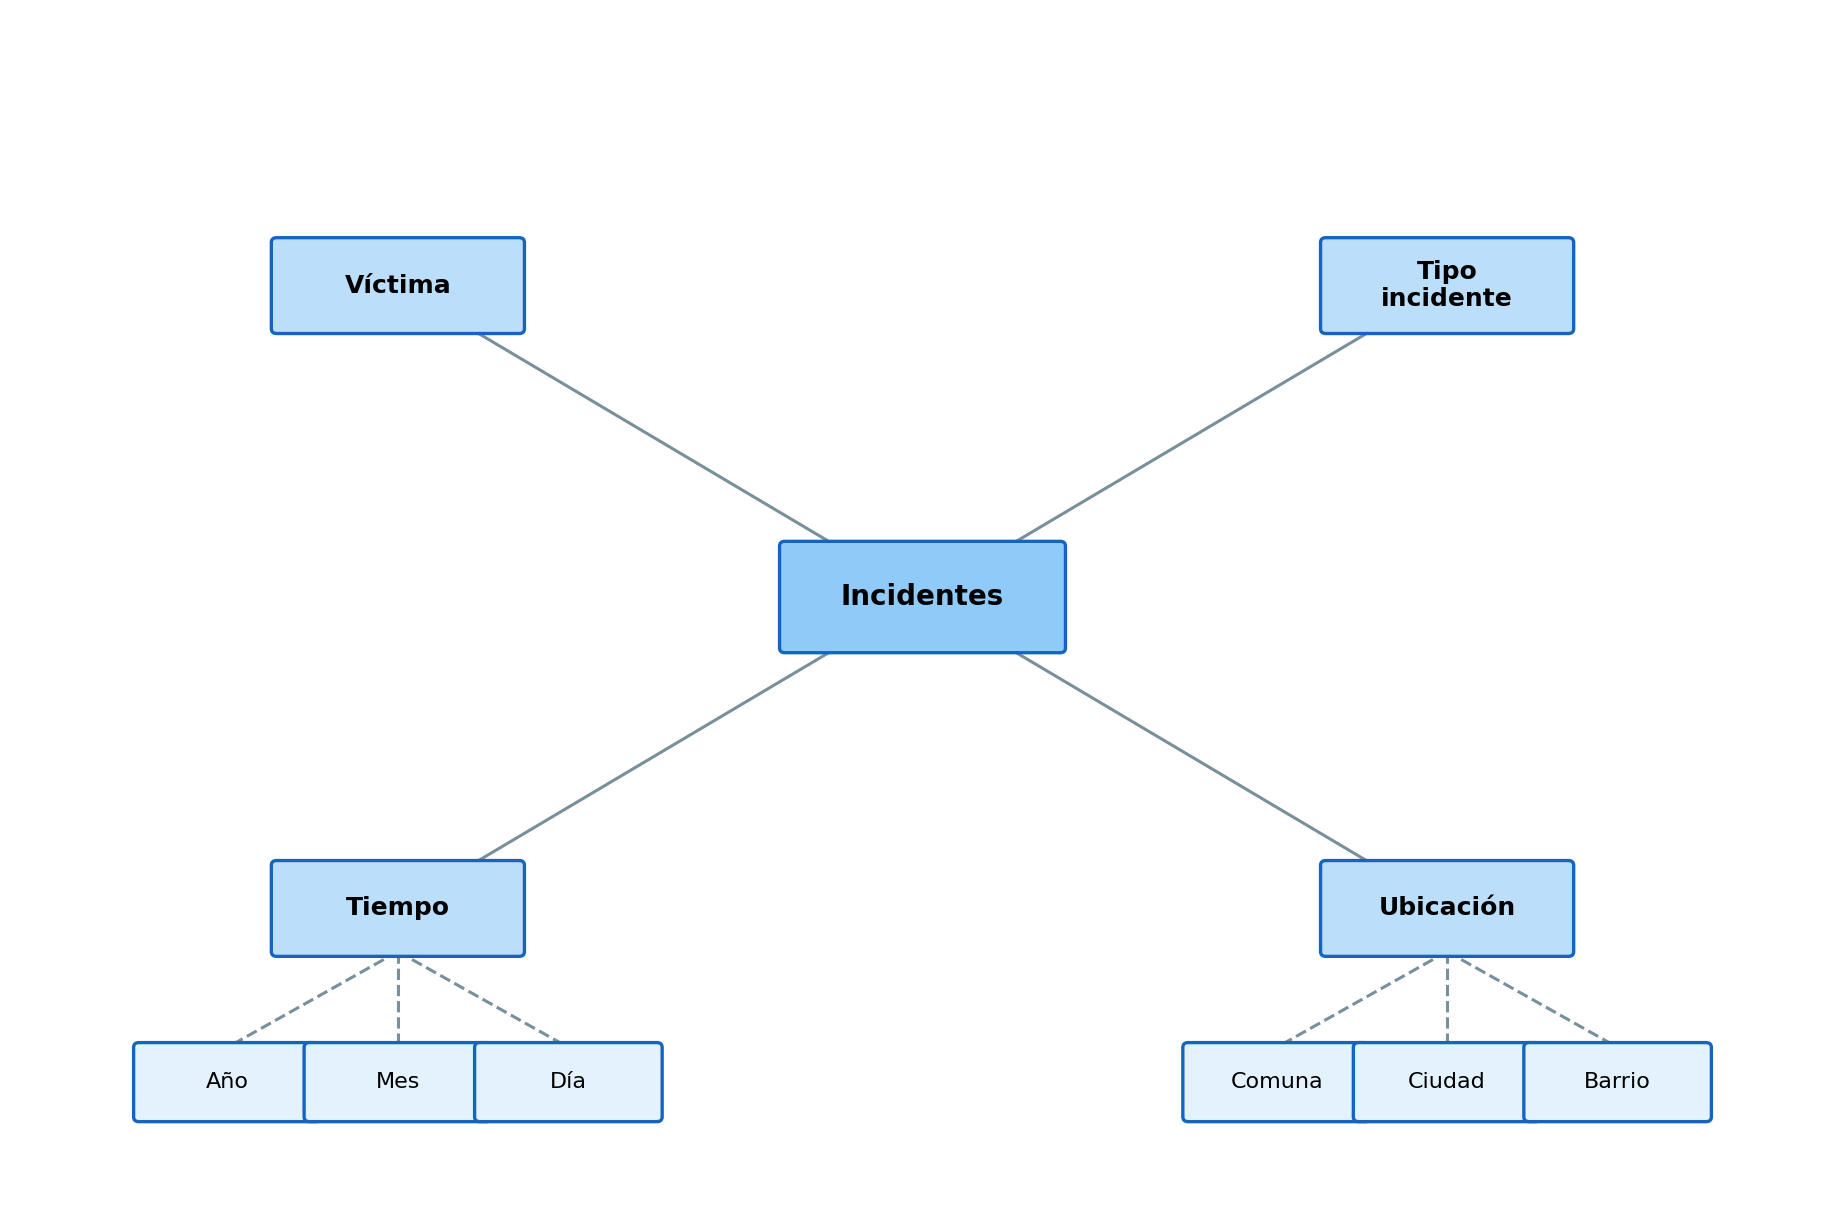
\includegraphics[width=0.85\linewidth]{images/fig_modelo_copo_nieve.png}
	\caption{Modelo copo de nieve aplicado a incidentes y dimensiones}
	\label{fig:arquitectura-monolitica-pagina-6}
\end{figure}

\subsection{Visualización analítica, tableros y experiencia de usuario}
Los dashboards integran gráficos, mapas y tablas dinámicas bajo filtros compartidos (fechas, territorio, clase, gravedad). La analítica visual apoya la decisión en entornos urbanos con información abundante y heterogénea \cite{monar2025}. En ViaData — Medellín, \textbf{mapas de calor, rankings territoriales, hotspots y series temporales} permiten detectar patrones y focalizar intervenciones. Los contratos de \textbf{API} conservan la misma semántica de indicadores en tablero, mapa, predicciones y asistente, de modo que un mismo filtro territorial produce resultados comparables entre módulos.

\subsection{Calidad y gobernanza de los datos}
La efectividad de la plataforma depende de la calidad del dato: estandarización, consistencia, trazabilidad desde Mede hasta el indicador expuesto y documentación de reglas de depuración en un único módulo ETL. Sin indicadores estructurados y gobernanza, los sistemas analíticos difícilmente sostienen políticas de seguridad vial basadas en evidencia \cite{oviedo2025,oms2024}. En ViaData — Medellín, la gobernanza se traduce en validación y normalización a catálogos, integridad referencial en la base, contraste registro--espacial (G03) y procesos de carga reproducibles, de modo que la plataforma funcione como infraestructura de conocimiento y no solo como reportes aislados.
